%======================== USD Thesis Template ==============================%
% Made according to the guide, keeping in mind the guide was made for Word
% TODO: Make a copy of this file that can be used right away once everything is done
\documentclass[oneside,12pt]{book}


\usepackage{titlesec} % Manage chapter and sections
\usepackage{fontspec} % Manage fonts
\usepackage{fancyhdr} % Manage header styles
\usepackage{lipsum} % Lorem Ipsum
\usepackage{graphicx} % to add images
\usepackage[portrait, left=4cm, right=3cm, top=3cm, bottom=3cm]{geometry} % set margins
\usepackage{indentfirst} % indents first line after section
\usepackage{setspace}
\usepackage{tocloft} % TOC modifications
\usepackage{listings} % Allow writing code
\usepackage{courier} % Code listing font family
\usepackage{import} % used to import files from different directories
\usepackage{float} % Adds more image float positions
\usepackage{pythontex} % Because
\usepackage[numbib]{tocbibind}
\usepackage[labelfont=bf, labelsep=period]{caption} % Manages captions. Changed to bold and separated using period
\usepackage{pdfpages} % Allows adding pdfs as pages
\usepackage{caption} % Used to create custom caption groups
\usepackage{amsmath} % Package for math
\usepackage{scrwfile} % used to edit the appendix toc
\usepackage{hyperref} % Hyperlink for references
\usepackage[toc, titletoc]{appendix} % For appendix-related things. Still not sure how to use it
\usepackage{pgfplots} % For plotting graphs
\usepackage{etoolbox} % Patching commands



%============================ Title details =================================%
\def\title{An Example of Skripsi Made Using \LaTeX}
\def\author{Echa}
\def\nim{080989999}
\def\prodi{Informatika}
\def\fakultas{Sains dan Teknologi}
\def\sarjana{Komputer}


%============================= Document Imports =============================%

%============================= Citations ====================================%
% Needs to make sure why \parencite doesn't return an author-year format
% 	Solved. No need to use \parencite*, use regular \parencite
\usepackage[
	style=apa
	]
	{biblatex}

\addbibresource{examplecitations.bib}

%============================ Fonts ======================================%
\setmainfont{Times New Roman}


%========================== Page Numbering =================================%
% Use fancyhdr styles
\pagestyle{fancy}

% Header settings
\fancyhead[L, C]{} 									% Resets the left and center header to show nothing
\renewcommand{\headrulewidth}{0pt} 					% removes the header line
\fancyhead[R]{\thepage} 							% Shows page number on the right side of header. \thepage is the page number variable

% Footer settings
\fancyfoot{}				 						% Clears settings
\fancyfoot[L]{Made by Hersa} 						% shows up even if page doesn't have numbering

% alter chapter-page numbering
\fancypagestyle{plain}{								% In fancyhrd, chapter pages use the plain style. Modify this to modify page numbering for chapter pages
	\fancyhf{} % resets page numbering for plain style
	\fancyfoot[R]{\thepage} % sets page number to the top right of the page

}


%=================== Chapter numbering =====================%
\renewcommand{\chaptermark}[1]{\markboth{#1}{}}

\renewcommand{\thesection}{\arabic{chapter}.\arabic{section}}

\titleformat % used to edit titles with titlesec
	{\chapter} % which command to edit
	[display] % shape
	{\bfseries\Large\centering} % format of the title
	{\uppercase{Bab} \thechapter} % label
	{0.5ex} % seperator
	{\uppercase} % before-code
	[\vspace{-0.5ex}] % after-code

\titlespacing{\chapter}{0pt}{0pt}{20pt} % Adjusts chapter title margin


%================== Quote modifications =============%
\renewenvironment{quote} {% Quotes are internally lists, somehow. Probably unmarked list
	\list{}{%
		\leftmargin0.5in   % this is the adjusting margin
		\rightmargin0cm
	}
	\item\relax
}
{\endlist}

%============= Table of contents modifications ==========%
% TODO: - Add chapter label to table of contents.
% TODO: - Make TOC entries uppercase and not bold.
% TODO: - Change filler to be more dots
% Create new list of lampiran using tocloft
\newcommand{\listlampiranname}{\hfill \Large DAFTAR LAMPIRAN \hfill}
\newlistof{lampiran}{lmp}{\listlampiranname}
\newcommand{\lampiran}[1]{ %
	\refstepcounter{lampiran}
	\par\noindent\textbf{Lampiran \thelampiran: #1}
	\addcontentsline{lmp}{lampiran}{\protect\numberline{\thelampiran} {#1}}
	\par
}

\newcommand{\listlistingname}{\hfill \Large DAFTAR LISTING \hfill}
\newlistof{listing}{ltsg}{\listlistingname}
\newcommand{\listing}[1]{
	\refstepcounter{listing}
	\par\noindent{\hfill \textbf{Listing}. #1}
	\addcontentsline{lstg}{listing}{\protect\numberline{\thelisting} {#1}}
}

\setcounter{tocdepth}{0}											% Sets depth of entries shown on ToC. 0 means only up to chapters


%***** ToC title modifications
\renewcommand{\contentsname}{DAFTAR ISI}							% Changes ToC title
\renewcommand{\listfigurename}{DAFTAR GAMBAR}
\renewcommand{\lstlistlistingname}{DAFTAR LISTING}
\renewcommand{\listtablename}{DAFTAR TABEL}

\renewcommand{\cfttoctitlefont}{\hfill\Large\bfseries}				% Changes style of ToC title. Sets left side to fill horizontal, Large font, bold
\renewcommand{\cftaftertoctitle}{\hfill}							% Sets to fill horizontal so the text is in the middle
\renewcommand{\cftloftitlefont}{\hfill\Large\bfseries}				% Figures
\renewcommand{\cftafterloftitle}{\hfill}
\renewcommand{\cftlottitlefont}{\hfill\Large\bfseries}				% Tables
\renewcommand{\cftafterlottitle}{\hfill}



% TODO List of listing still not working with tocloft

%****** TOC ENTRY MODIFICATIONS *******

%***** TOC
% Makes it so tocloft chapter accepts argument
\makeatletter
\patchcmd{\l@chapter}
{\cftchapfont #1}%   search pattern
{\cftchapfont {#1}}% replace by
{}%                  success
{}%                  failure
\makeatother


\renewcommand{\cftchappresnum}{BAB } 						% Adds the word "BAB " before toc chapter numbering
\setlength\cftchapnumwidth{3.8em} 							% sets width of number box (adjusted so number doesn't overlap with chapter naming). If chapter has no number, then doesn't add word
\renewcommand{\cftchapdotsep}{1} 							% Sets distance between dots
\renewcommand{\cftchapleader}{\cftdotfill{\cftchapdotsep}}	% Adds dots to chapter entry on toc
\renewcommand\cftchapfont{\uppercase}						% Sets TOC entries as uppercase
\renewcommand\cftchappagefont{}								% Sets font for the entries. Left empty so it removes bold. Can be adjusted for size

%***** Figures
\makeatletter
\patchcmd{\l@figure}
{\cftfigfont #1}
{\cftfigfont {#1}}
{}{}
\makeatother

\renewcommand{\cftfigpresnum}{GAMBAR }
\setlength{\cftfignumwidth}{7em}
\renewcommand{\cftfigdotsep}{1}
\renewcommand{\cftfigleader}{\cftdotfill{\cftfigdotsep}}
\renewcommand{\cftfigfont}{\uppercase}
\renewcommand{\cftfigpagefont}{}
\renewcommand{\cftfigindent}{0pt}


%***** Tables
\makeatletter
\patchcmd{\l@table}
{\cfttabfont #1}
{\cfttabfont {#1}}
{}{}
\makeatother

\renewcommand{\cfttabpresnum}{TABEL }
\setlength{\cfttabnumwidth}{6em}
\renewcommand{\cfttabdotsep}{1}
\renewcommand{\cfttableader}{\cftdotfill{\cfttabdotsep}}
\renewcommand{\cfttabfont}{\uppercase}
\renewcommand{\cfttabpagefont}{}
\renewcommand{\cfttabindent}{0pt}

%***** Listing
% TODO:


%***** Lampiran
\makeatletter
\patchcmd{\l@lampiran}
{\cftlampiranfont #1}
{\cftlampiranfont {#1}}
{}{}
\makeatother

\renewcommand{\cftlampiranpresnum}{LAMPIRAN }
\setlength{\cftlampirannumwidth}{7em}
\renewcommand{\cftlampirandotsep}{1}
%%\renewcommand{\cftlampiranleader}{\cftdotfill{\cftlampirandotsep}}
\renewcommand{\cftlampiranfont}{\uppercase}
\renewcommand{\cftlampiranpagefont}{}
\renewcommand{\cftlampiranindent}{0pt}


%=================== Appendix modifications ===============%
% Create new environment for appendix
% source: https://tex.stackexchange.com/questions/184103/how-to-define-a-custom-environment-caption-for-table-of-contents


%================== Graph Modifications
\pgfplotsset{width=10cm, compat=1.9}

\usepgfplotslibrary{external}



%============= Caption label modifications ==============%
\renewcommand{\figurename}{Gambar}
\renewcommand{\tablename}{Tabel}


\captionsetup[table]{singlelinecheck=false}

\renewcommand{\thetable}{\arabic{chapter}.\arabic{table}}
\AtBeginDocument{
	\renewcommand{\thelstlisting}{\arabic{chapter}.\arabic{lstlisting}}
}
\renewcommand{\thefigure}{\arabic{chapter}.\arabic{figure}}
%================== Code block modifications =============%
% TODO: Maybe find a way to add colors
\lstset{numbers=left, numberstyle=\tiny}
\lstdefinestyle{skripsilisting}{numbers=left, numberstyle=\tiny, lineskip=-0.8ex, basicstyle=\small}

%================ Start of document ==================%
\begin{document}

%================== Custom title page ================%
% TODO: Check if title page is correct or not
\begin{titlepage}
	\begin{center}
		\large
		\textbf{\MakeUppercase{\title}}
		\vspace{2ex}


		\textbf{SKRIPSI}

		\vspace{2ex}

		Diajukan untuk memenuhi salah satu syarat memeroleh gelar Sarjana \sarjana \\Program Studi \prodi


		\vspace{3cm}
		
\includegraphics[width=5cm]{usd}\\
		\vspace{1.5cm}
		Disusun oleh:\\
		\author\\
		NIM: \nim\\

		\vspace{2cm}

		\MakeUppercase{
			Fakultas \fakultas\\
			Universitas Sanata Dharma\\
			Indonesia\\
			\the\year{}\\
		}
	\end{center}
\end{titlepage}

%=================== Front matters =======================%
% Bastracts, page of thanks, table of content/figures/etc
\frontmatter

% uses \addcontentsline to add PDF into TOC. Should add the line before adding the PDF so it's on the same page as the start of PDF
\addcontentsline{toc}{chapter}{Inserted PDF}
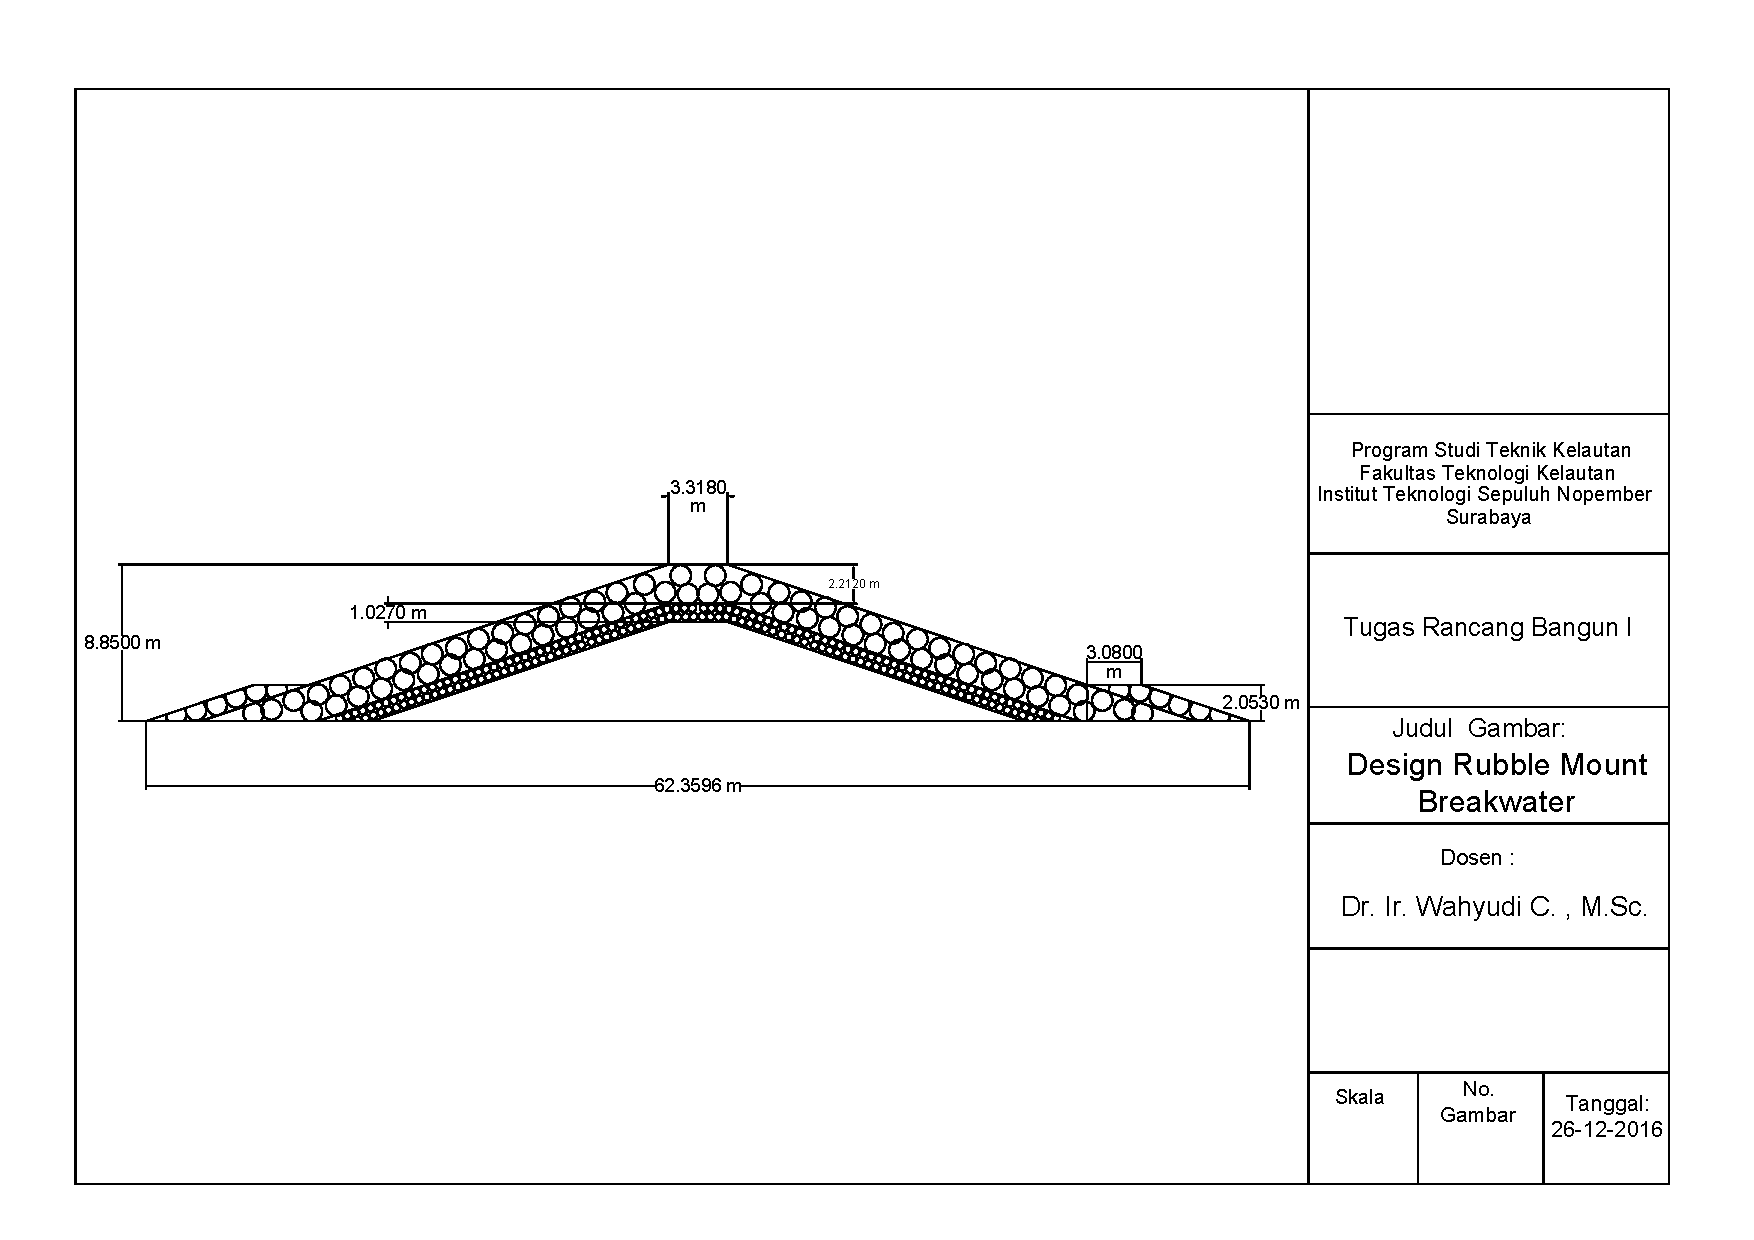
\includepdf{Breakwater.pdf}


\chapter{Kata Pengantar}

\chapter{Abstrak}

\chapter{Abstract}

\renewcommand{\thechapter}{\Roman{chapter}} % Makes chapter numbering roman numeral
\clearpage
\tableofcontents

\renewcommand{\thechapter}{\arabic{chapter}} % Makes chapter numbering roman numeral
\clearpage
\listoffigures

\clearpage
\listoftables

\clearpage
\lstlistoflistings

\clearpage
\addcontentsline{toc}{chapter}{Daftar Lampiran}
\listoflampiran
\renewcommand{\thechapter}{\Roman{chapter}} % Makes chapter numbering roman numeral



%=================== Main part of document =================%
% Chapters etc
% TODO: Check if spacing is correct
\mainmatter

\begin{doublespace}

% \spacing{1.213}
% Pendahuluan - Importing from subdirectory
\subimport{Skripsi/Pendahuluan}{pendahuluan}

% Landasan Teori
\subimport{Skripsi/Landasan_Teori}{landasan_teori}

% Importing from the same directory
\chapter{Code Examples}

\section{Writing code directly to LaTeX}
\begin{lstlisting}[caption=Manual input, label={listing-java-manual},language=java,style=skripsilisting]
	public class HelloWorld {
		public static void main(String[] args) {
			System.out.println("Hello world");
		}
	}
\end{lstlisting}

\section{Importing code}

\lstinputlisting[caption=Test java, label={lst:listing-java}, language=java, style=skripsilisting]{Mahasiswa.java}


\chapter{Another file in another folder}
Well well well, what do we have here?. Use this command in the document body to insert the contents of another file named filename.tex; again this file should not contain any LATEX preamble. LATEX will start a new page before processing the material input from filename.tex. Make sure not to include the extension .tex in the filename, as this will stop the file from being input (the extension can optionally be included with input and import). It is not possible to nest include commands. Each file that gets has its own .aux file storing information of created labels and contents for the table of contents, list of figures, etc. You can use  with a comma separated list of file names (make sure that there are no leading or trailing spaces). If you do this LATEX will only process the files contained in that list. This can be used to enhance compilation speed if you're only working on a small part of a bigger document. Page numbers and cross references will however still work, as the .aux files of left out files will still be processed.
\section{Title}
\lipsum[1-2]


\subimport{New_Chapter}{another_one} % Imports from subdirectory


\end{doublespace}
%================= Back matters ===================%
% Bibliography and attachments/appendices

\backmatter

\printbibliography[heading=bibintoc, title=DAFTAR PUSTAKA]


\clearpage
\appendix
\addcontentsline{toc}{chapter}{Lampiran}
\lampiran{Kode dalam Lampiran}\begin{lstlisting}[label={listing-java-manual},language=java,style=skripsilisting]
	public class HelloWorld {
		public static void main(String[] args) {
			System.out.println("Hello world");
		}
	}
\end{lstlisting}



\end{document}



